\documentclass[tikz, crop, border=5pt]{standalone}
\usetikzlibrary{positioning,backgrounds,fit,shapes.geometric,calc}

\usepackage{fontspec}
\usepackage{xeCJK}

\setmainfont{NotoSans}[
    Extension      = .ttf,
    UprightFont    = *-Regular,
    BoldFont       = *-Bold,
    ItalicFont     = *-Italic,
    BoldItalicFont = *-BoldItalic
]

\usepackage{color}
%COLOR_BEGIN%
\definecolor{black}{RGB}{26,25,25}
\definecolor{grey}{RGB}{129,130,132}
\definecolor{red}{RGB}{188,36,46}
\definecolor{brown}{RGB}{121,37,0}
\definecolor{green}{RGB}{32,128,108}
\definecolor{purple}{RGB}{160,90,150}
\definecolor{blue}{RGB}{0,103,149} % MidnightBlue
%COLOR_END%

\tikzset{
    base/.style={
        draw=grey,
        fill=grey,
        text=white,
    },
    % Adenylation
    A/.style={
        base,
        circle,
        minimum size=1cm,
        inner sep=0pt,
        anchor=south,
        yshift=-2mm,
    },
    % Condensation
    C/.style={
        base,
        regular polygon,
        regular polygon sides=3,
        shape border rotate=180,
        minimum width=0.9cm,
        inner sep=0pt,
        anchor=north,
        yshift=1mm,
    },
    % Epimerization
    E/.style={
        base,
        regular polygon,
        regular polygon sides=3,
        shape border rotate=0,
        minimum width=0.9cm,
        anchor=south,
        yshift=-1mm,
    },
    % Condensation/Epimerization
    CE/.style={
        base,
        diamond,
        minimum width=0.8cm,
        minimum height=1.19cm,
    },
    % Thiolation
    T/.style={
        base,
        rectangle,
        minimum height=0.4cm,
        minimum width=0.2cm,
        anchor=north,
    },
    % Thioesterase
    Te/.style={
        base,
        circle,
        minimum width=0.6cm,
        anchor=north,
        yshift=2mm,
    },
    % Reductase
    R/.style={
        base,
        regular polygon,
        regular polygon sides=4,
        minimum width=0.8cm,
        anchor=north,
        yshift=2mm,
    },
    % Methyltransferase
    M/.style={
        base,
        ellipse,
        minimum width=0.9cm,
        minimum height=0.6cm,
    },
}

\begin{document}
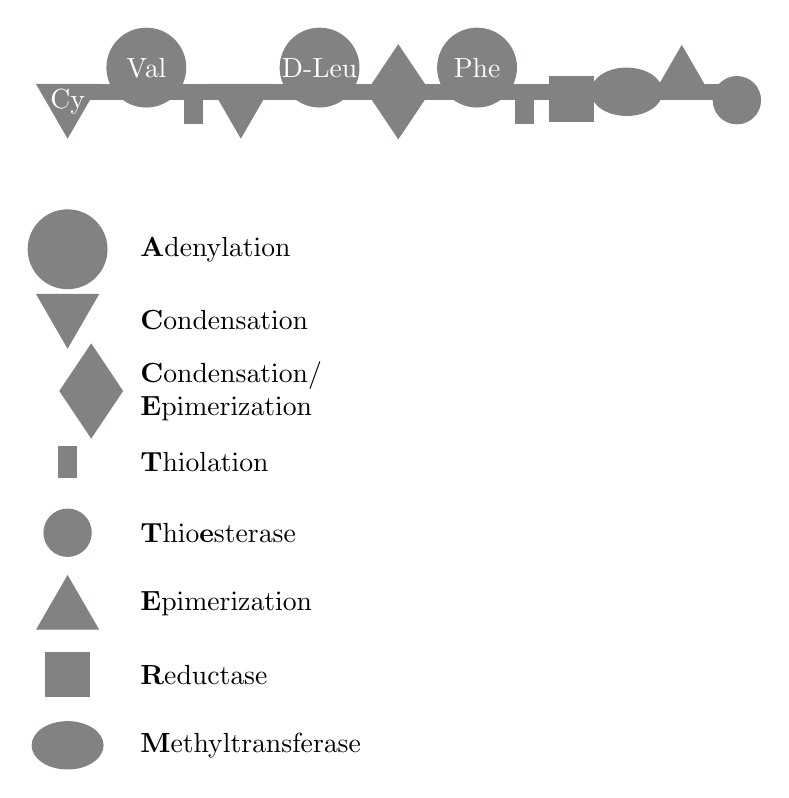
\begin{tikzpicture}
%MODULE_BEGIN%
    \node[C] (c1) at (0,0) {};
    \node[text=white] at (c1) {Cy};
    \node[A] at (1,0) {Val};
    \node[T] at (1.6,0) {};
    \node[C] at (2.2,0) {};
    \node[A] at (3.2,0) {D-Leu};
    \node[CE] at (4.2,0) {};
    \node[A] at (5.2,0) {Phe};
    \node[T] at (5.8,0) {};
    \node[R] at (6.4,0) {};
    \node[M] at (7.1,0) {};
    \node[E] at (7.8,0) {};
    \node[Te] at (8.5,0) {};
    % Draw module sequence
    \begin{scope}[on background layer]
        \draw[grey, line width=2mm] (0,0) -- (8.5,0);
    \end{scope}
%MODULE_END%

%LEGEND_BEGIN%
    \begin{scope}[yshift=-2cm]
        \begin{scope}[yshift=0cm]
            \node[A,anchor=center,yshift=2mm,] at (0,0) {};
            \node[anchor=west] at (0.8,0) {\textbf{A}denylation};
        \end{scope}

        \begin{scope}[yshift=-0.9cm]
            \node[C,anchor=center] at (0,0) {};
            \node[anchor=west] at (0.8,0) {\textbf{C}ondensation};
        \end{scope}

        \begin{scope}[yshift=-1.8cm]
            \node[CE] at (0.3,0) {};
            \node[anchor=west,align=left] at (0.8,0) {\textbf{C}ondensation/\\\textbf{E}pimerization};
        \end{scope}

        \begin{scope}[yshift=-2.7cm]
            \node[T,anchor=center] at (0,0) {};
            \node[anchor=west] at (0.8,0) {\textbf{T}hiolation};
        \end{scope}

        \begin{scope}[yshift=-3.6cm]
            \node[Te,anchor=center,yshift=-2mm,] at (0,0) {};
            \node[anchor=west] at (0.8,0) {\textbf{T}hio\textbf{e}sterase};
        \end{scope}

        \begin{scope}[yshift=-4.5cm]
            \node[E,anchor=center] at (0,0) {};
            \node[anchor=west] at (0.8,0) {\textbf{E}pimerization};
        \end{scope}

        \begin{scope}[yshift=-5.4cm]
            \node[R,anchor=center,yshift=-2mm] at (0,0) {};
            \node[anchor=west] at (0.8,0) {\textbf{R}eductase};
        \end{scope}

        \begin{scope}[yshift=-6.3cm]
            \node[M] at (0,0) {};
            \node[anchor=west] at (0.8,0) {\textbf{M}ethyltransferase};
        \end{scope}
    \end{scope}
%LEGEND_END%
\end{tikzpicture}
\end{document}
